\documentclass[a4paper]{article}
\usepackage[warn]{mathtext}
\usepackage[utf8]{inputenc}
\usepackage[T2A]{fontenc}

\usepackage[english,russian]{babel}
\usepackage{multicol}
\usepackage{fancyhdr}
\usepackage{graphicx}
\usepackage{microtype}
\usepackage{wrapfig}
\usepackage{amsmath}
\usepackage{floatflt}
\usepackage{geometry} \geometry{verbose,a4paper,tmargin=2cm,bmargin=2cm,lmargin=1.5cm,rmargin=1.5cm}
\usepackage{float}
\usepackage{amssymb}
\usepackage{caption}
\usepackage{epsfig}
\usepackage{newunicodechar}

\begin{document}

\graphicspath{ {pictures/} }

\begin{titlepage}
	\centering
	\vspace{5cm}
    {\scshape\LARGE Московский физико-технический институт\par}
	\vspace{5cm}
	{\scshape\Large Лабораторная работа по общей физике \par}
	\vspace{1cm}
    {\huge\bfseries  №11.1 Определение ширины запреженной зоны полупроводника  \par}
	\vspace{1cm}
	\vfill
    \begin{flushright}
        {\large выполнил студент Б04-852 группы ФЭФМ}\par
        \vspace{0.3cm}
        {\LARGE Яромир Водзяновский}
    \end{flushright}
	\vfill
Долгопрудный, 2021
% Bottom of the page
\end{titlepage}

\pagestyle{fancy} 
\fancyhead[L]{Полупроводник    $\sim  \hat(\, ^{\circ}  \omega  ^{\circ} \, \hat) \sim$}
% \fancyhead[L]{Закон Кюри-Вейса    $( *{^\circ}< >^{\circ}*)$}
\fancyhead[R]{Современная физика}
\fancyhead[C]{}
\fancyfoot[C]{ \noindent\rule{\textwidth}{0.4pt} \thepage }

\tableofcontents

\newpage



\section{Цель работы}

\begin{itemize}
    
\item Исследовать температурную зависимость проводимости типичного полупроводника - германия или кремния
\item Определить ширину запрещенной зоны 2-мя методами: постоянный ток и переменный ток.
\end{itemize}



\section{Теория}

Величина электропроводности в полупроводниках определяется числом электронов в зоне проводимости и дырок в 
валентной зоне. \par 

ЧИсло электронов в зоне проводимости равно произведению числа имеющихся уровней на вероятность их заполнения, определяется это функцие Ферми, 
в нашем случае мало отличается от больцмановского распределния: 

\begin{equation}
    f(E) = \frac{1}{e^{\frac{E - \mu}{k_b T}}+1} \approxeq e^{- \frac{E - \mu}{k_b T}}
\end{equation}

$E$ - энергия уровня в зоне проводимости, $\mu$ - энергия Ферми, лежит вблизи середины запрещенной зоны. \par 

\begin{figure}[H]
    \begin{center}
        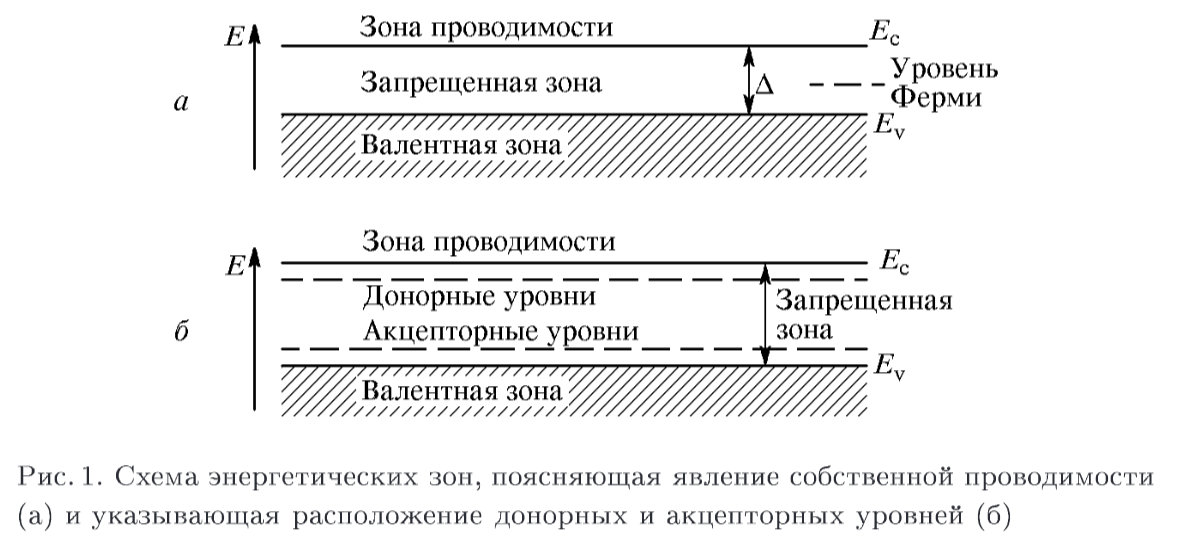
\includegraphics[scale = 0.5]{p1.png}
        \caption{}
        \label{p1}
    \end{center}
\end{figure}


Вместо полного числа уровней в зоне подставим эффективное значение $Q_n$, вблизи дна зоны, то число жлектронов в зоне проводимости:

\begin{equation}
    n_n = Q_n e^{- \frac{E_x - \mu}{k_b T}}
\end{equation}

Вероятность появления дырки $1-f(E)$, то число дырок:

\begin{equation}
    n_p = Q_p \left[ 1 - \frac{1}{e^{\frac{E_v - \mu}{k_bT}}+1} \right] =\approxeq Q_p e^{- \frac{E_v - \mu}{k_b T}}
\end{equation}


Получим, что число электронов равно числу дырок:

\begin{equation}
    n_n n_p = n^2 = Q_n Q_p e^{- \frac{E_v - \mu}{k_b T}}
\end{equation}

Знаем, что $E_c - E_v = \Delta$, $Q_n Q_p = C^2$

Получим:

\begin{equation}
    n = C e^{- \frac{\Delta}{2 k_b T}}
\end{equation}

Электропроводность полупроводника? В поле большая часть элекронов в зоне проводимости начинает двигаться в сторону, противоположную полю. 
Среднаяя скорость направлена вдоль поля:

\begin{equation}
    v_{ср} = \mu_n \varepsilon
\end{equation}

$\mu_n$ - подвижность электронов, $v_{ср}$ -  средняя дрейфовая скорость. \par 

Найдем проводимость через ф-лу $j = nev_{ср}$:

\begin{equation}
    \sigma = j \varepsilon  = |e| (n_n \mu_n + n_p \mu_p)
\end{equation}

Тк $n_n = n_p$:

\begin{equation}
    \sigma = |e|C(\mu_n + \mu_p) e^{- \frac{\Delta}{2k_b T}} = A e^{- \frac{\Delta}{2k_b T}}
\end{equation}

Все рассуждения верны, тк электропроводность полупроводника опредяляется переходами электронов из валентной зоны в зону проводимости - это вклад собственной провдимости полупроводника. 
При низких температурах вклад уже вносят примесная проводимость.  \par  

Примесная проводимость искажает температурный ход собственной электропроводности. Чтобы определить ширину запреженной зоны надо провести исследование в шировокм интервале температур, где электропроводность от 1/T
имеет экспоненциальный характер. 


\section{Экспериментальные установки}

\subsection{Исследование зависимости $\sigma(T)$ с помощью универсального цифрового вольтметра В7-34А}

\begin{figure}[H]
    \begin{center}
        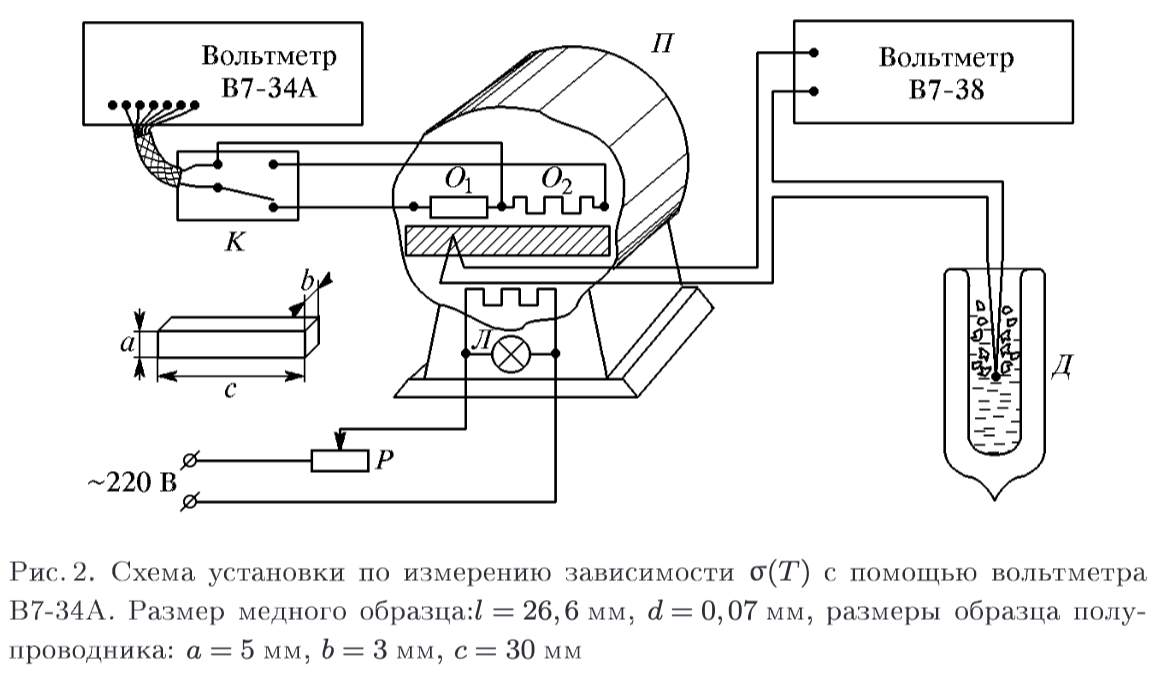
\includegraphics[scale = 0.5]{setup1.png}
        \caption{}
        \label{setup1}
    \end{center}
\end{figure}

На рис. \ref{setup1} изображена схема установки. Мы будем исследовать 2 образца $O_1$ и $O_2$. Погрешность при измерении сопротивлений не превышает:

\begin{equation}
    \pm [0.015 \pm 0.02 (R_k/R_x - 1)]
\end{equation}

$R_k$ - включенный предел измерений, $R_x$ - значение измеряемой величины в кОм. \par 

Ток через подключенный образец не превышает 1 мА. Один из образцов изготовлен из кристаллического германия и имеет форму прямоугльного параллилепипед, другой - из тонкой медной 
проволоки длиной около двадцати метров. 

\begin{equation}
    \sigma = \frac{l}{RS}
\end{equation}

Нагрев образцов регулируетяс реостатом Р. Один спай термопары термопары находится у оброзцов, другой в сосуде Дюара. 
Эдс термопары измеряетсмя вольтметром, постоянная термопары $41 \cdot 10^{-6}$ В/К. \par 

Нагрев надо провдить равномерно, чтобы была одинаковая температура по всей длине. Первый способ - быстрый нагрев вечи при максимайльной подводимой мощности 5 мин, затем выдержка 10 мин. 
Второй способ - медленный нагрев при малой мощности и, не выключая его, проводить измерения температуры и сопротивления образцов. 

\subsection{Исследование зависимости $\sigma(T)$ с помощью моста переменного тока.}

\begin{figure}[H]
    \begin{center}
        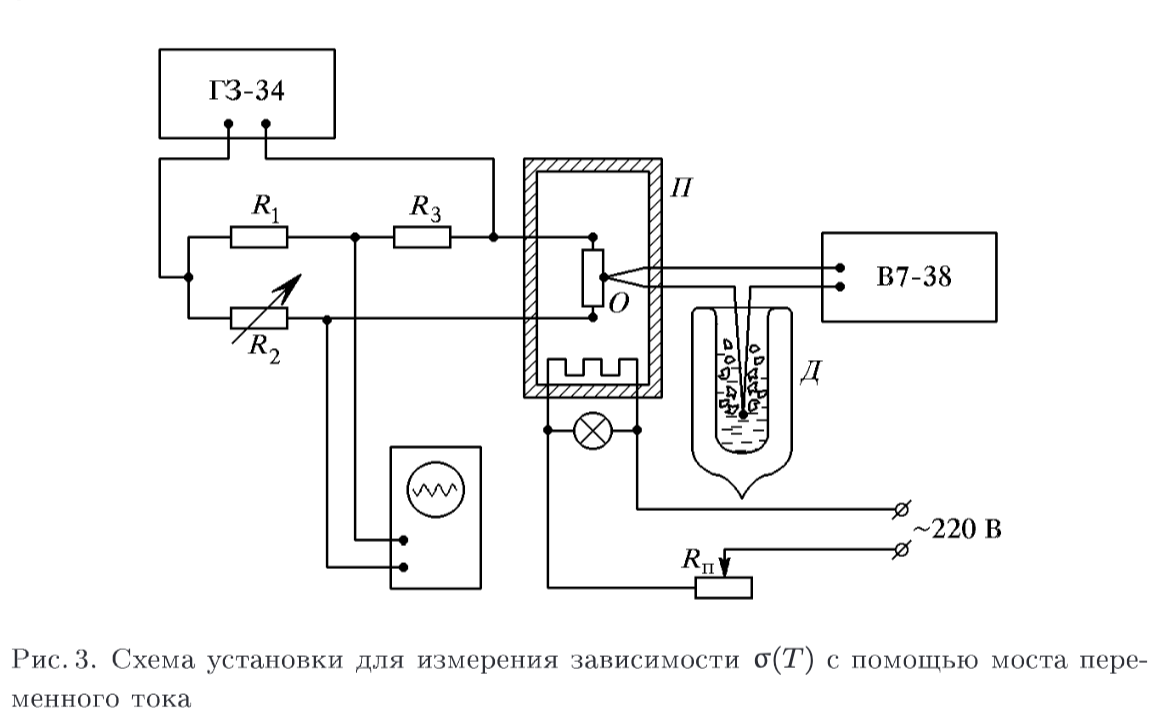
\includegraphics[scale = 0.5]{setup2.png}
        \caption{}
        \label{setup2}
    \end{center}
\end{figure}

Схема установки на рис. \ref{setup2}. Полупровдниковый образец это одно из плеч моста. другие плечи образую омические сопротивления. 
В качестве $R_2$ используется магазин сопротивлений. Мост питается от звукового генератора Г3-34. В качестве нуль гальвонометра используется осциллограф. 
Чтобы обеспечить равномерный нагревобразца его помещают в маслянную ванночку. Температура измеряется медь-константановой термопарой. 

\begin{equation}
    \sigma_x = \frac{l}{S} \frac{R_1}{R_3} \frac{1}{R_2}
\end{equation}

$R_2$ обеспечивает баланс моста. 




\section{Ход работы}


\subsection{Исследование зависимости $\sigma(T)$ с помощью универсального цифрового вольтметра В7-34А}

\begin{enumerate}
    \item Включим в сеть вольтметр и дадим ему прогреться, переведем его в режим измрения постоянного тока, подставим 
    реостат электропечи в средне положение и включим печь в сеть.

    \item Будем нагревать образцы от комнатной температуры до 100 $^{\circ} C$. Через каждые $10 ^{\circ} C$ будем измерять сопротивления образцов, поочередно подключая их к вольтметру. 
    \item По полученным данным (рис. \ref{data2}) построим зависимости для $\sigma(T)$ для меди (рис. \ref{gr5}) и полупроводника (рис. \ref{gr2})
    \item По наклону графика для медного образца (рис. \ref{gr5}) определим температурный коэффициент. 

    \begin{center}
        \fbox{$\alpha = - \frac{1}{\sigma} \frac{d \sigma}{d T} = (344.5 \pm 3.7) \cdot 10^{-5} \; (1/K)\; [\pm 1.1 \%]$}
    \end{center}

    Для меди табличное значение $\alpha \approx 4.3 \cdot 10^{-3} \; (1/K)$. Не очень точно у меня получилось.
 
    \item Построим график $\ln{\sigma} = f(1/T)$ (рис. \ref{gr4}) и по наклону определим ширину запрещенной зоны. 

        \begin{center}
            \fbox{$\Delta = -2k_b\cdot a = (748 \pm 7)\cdot 10^{-3} \; (эВ) \; [\pm 0.9\%]$}
        \end{center}
        
        Значение не очень близко к значению ширины запрещенной зоны для Германия $\Delta_{Ge} \approx 0.67\; эВ$

    \item Я сделал экспоненциальную аппроксимацию функцией уравнения (8) графика $\sigma(T)$ (рис. \ref{gr3}). По полученому параметру $a = -3821.37 \pm 43.69 \; (K)$:
    
        \begin{center}
            \fbox{$\Delta = -2k_b\cdot a = (659 \pm 8)\cdot 10^{-3} \; (эВ) \; [\pm 1.2\%]$}
        \end{center}

        Это значение уже ближе к <<правде>>.

\end{enumerate}



\subsection{Исследование зависимости $\sigma(T)$ с помощью моста переменного тока}

\begin{enumerate}
    \item Включим осциллограф в сеть, включим генератор и установим на выходе сигнал с амплитудой 1 В, частота $\sim 600\; Гц$.
    \item Мост мы будем балансировать с помощью магазина сопротивлений $R_2$ каждый раз, кога абудем снимать значения напряжения термопары.
    \item Проведем эксперимент в диапазне температур от комнатной до 110 $^{\circ}C$. Данные занесем в таблицу на рис. \ref{data}.
    \item Построим график $\sigma(T)$ (рис. \ref{gr2}) и по экспоненциальной аппроксимации (8) определим ширину запрещенной зоны,  по полученому параметру $a = -3724.08 \pm 16.34 \; (K)$:

        \begin{center}
            \fbox{$\Delta = -2k_b\cdot a = (642 \pm 3)\cdot 10^{-3} \; (эВ) \; [\pm 0.5\%]$}  
        \end{center}
        
        Получается достаточно близкое значение к действительному для Германия $\Delta_{Ge} \approx 0.67\; эВ$.
         
    \item Построим график $\ln{\sigma} = f (1/T)$ (рис. \ref{gr1}) и по наклону определим ширину запреженной зоны:

    \begin{center}
        \fbox{$\Delta = -2k_b\cdot a = (588 \pm 6)\cdot 10^{-3} \; (эВ) \; [\pm 1\%]$}  
    \end{center}

        Линейная аппроксимация не дает достаточно точного результата.

\end{enumerate}


\section{Вывод}
В данной работе мы:
\begin{enumerate}
    \item Исследовали температурную зависимость проводимости для меди и типичного полупроводника - германия.
    \item Определили температурный коэффициент проводимости для меди: $\alpha = (344.5 \pm 3.7) \cdot 10^{-5} \; (1/K)\; [\pm 1.1 \%]$.
    \item Определить ширину запрещенной зоны 2-мя методами: в режиме постоянного тока и с помощью моста переменного тока.
\end{enumerate}
    

\section{Графики и таблицы с данными}

\begin{figure}[h]
    \begin{center}
        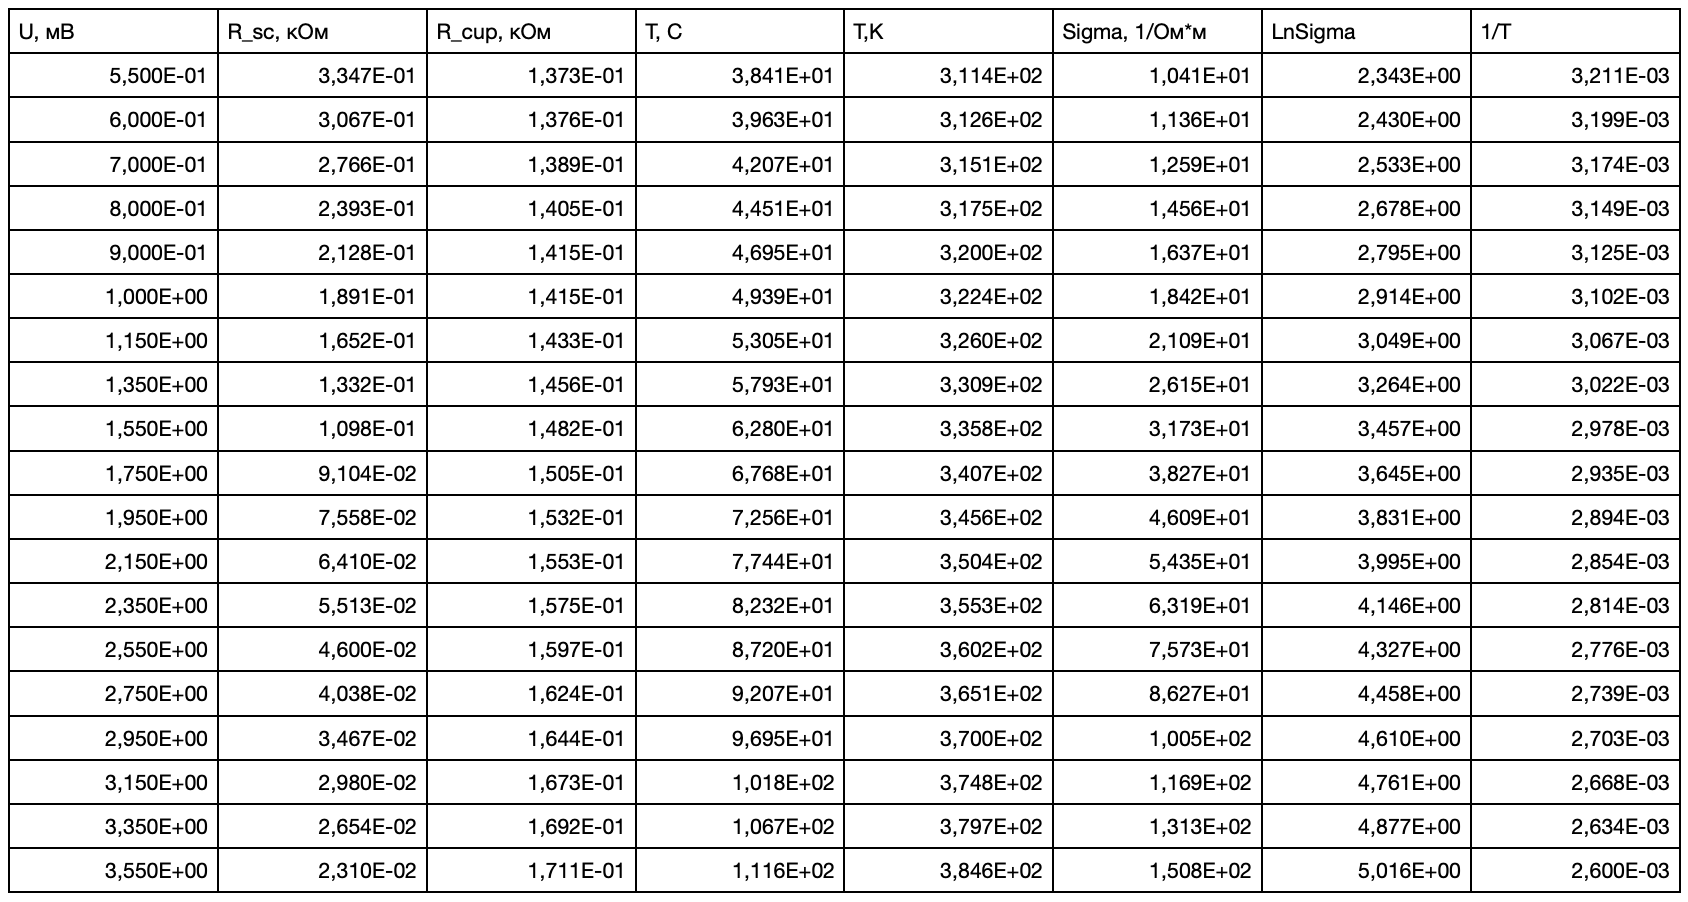
\includegraphics[scale = 0.55]{data2.png}
        \caption{Данные исследования в режиме постоянного тока.}
        \label{data2}
    \end{center}
\end{figure}

\begin{figure}[h]
    \begin{center}
        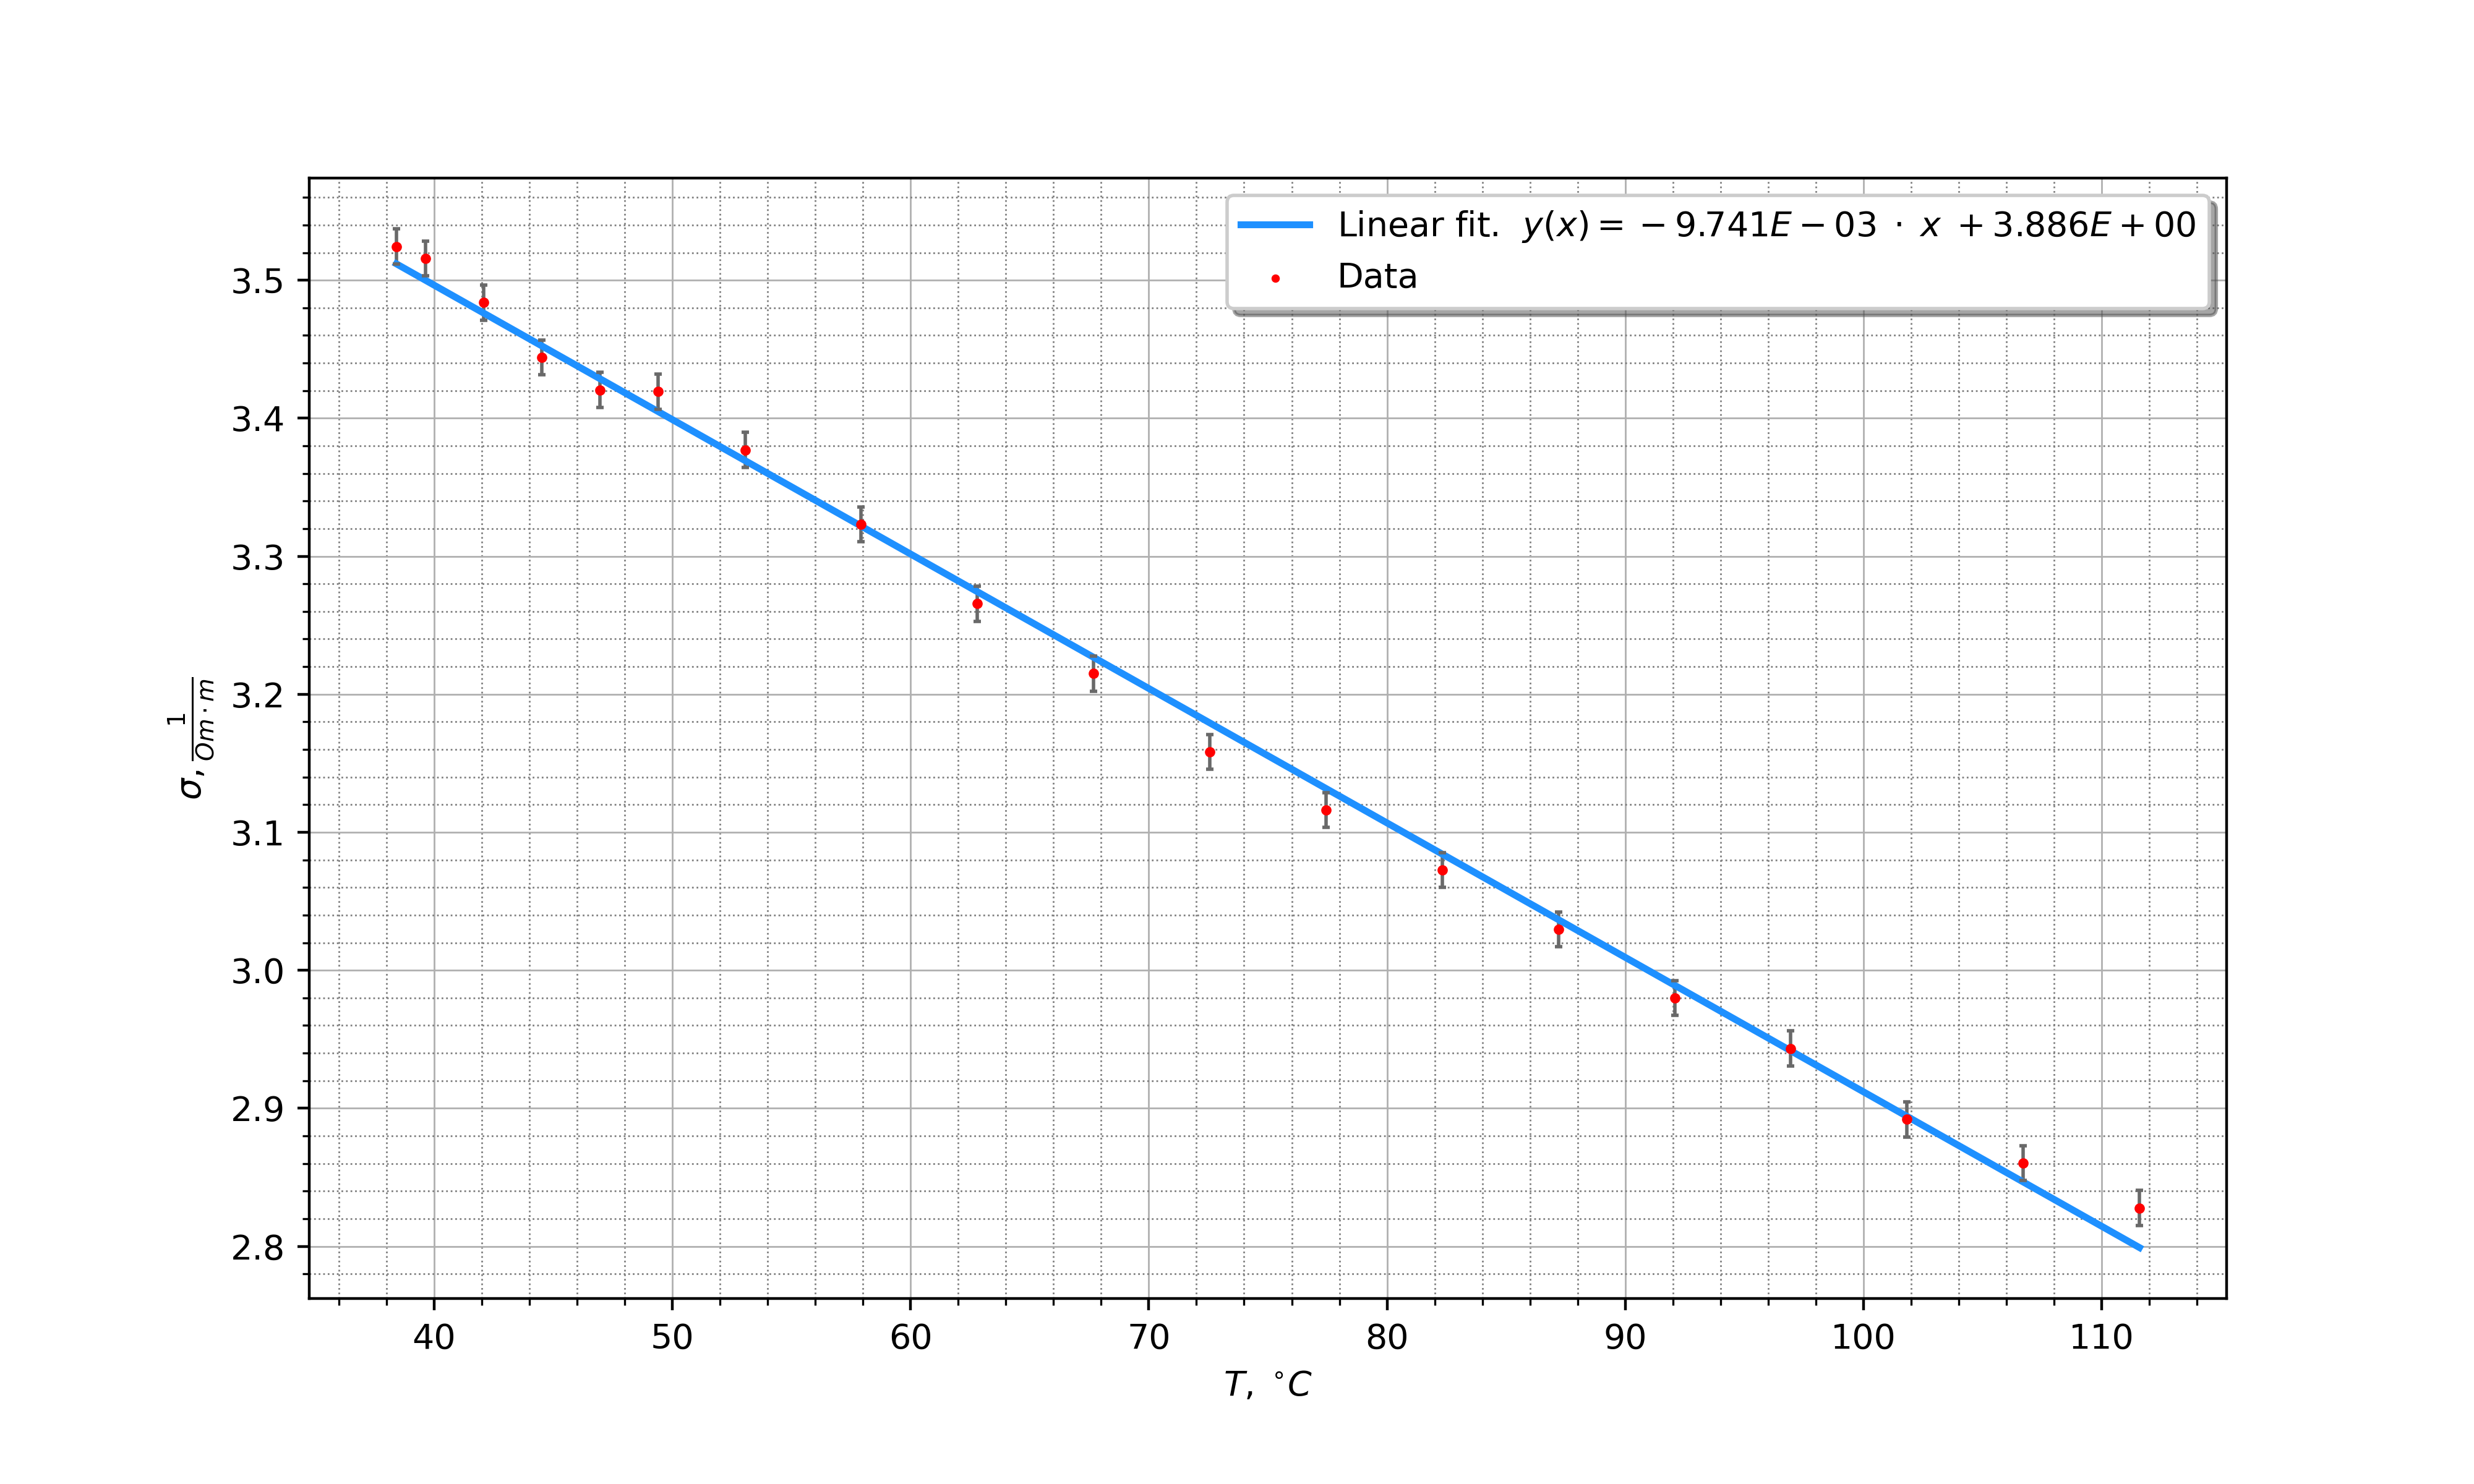
\includegraphics[scale = 0.75]{graph5.png}
        \caption{Зависимость $\sigma(T) $ для меди в режиме постоянного тока}
        \label{gr5}
    \end{center}
\end{figure}

\begin{figure}[h]
    \begin{center}
        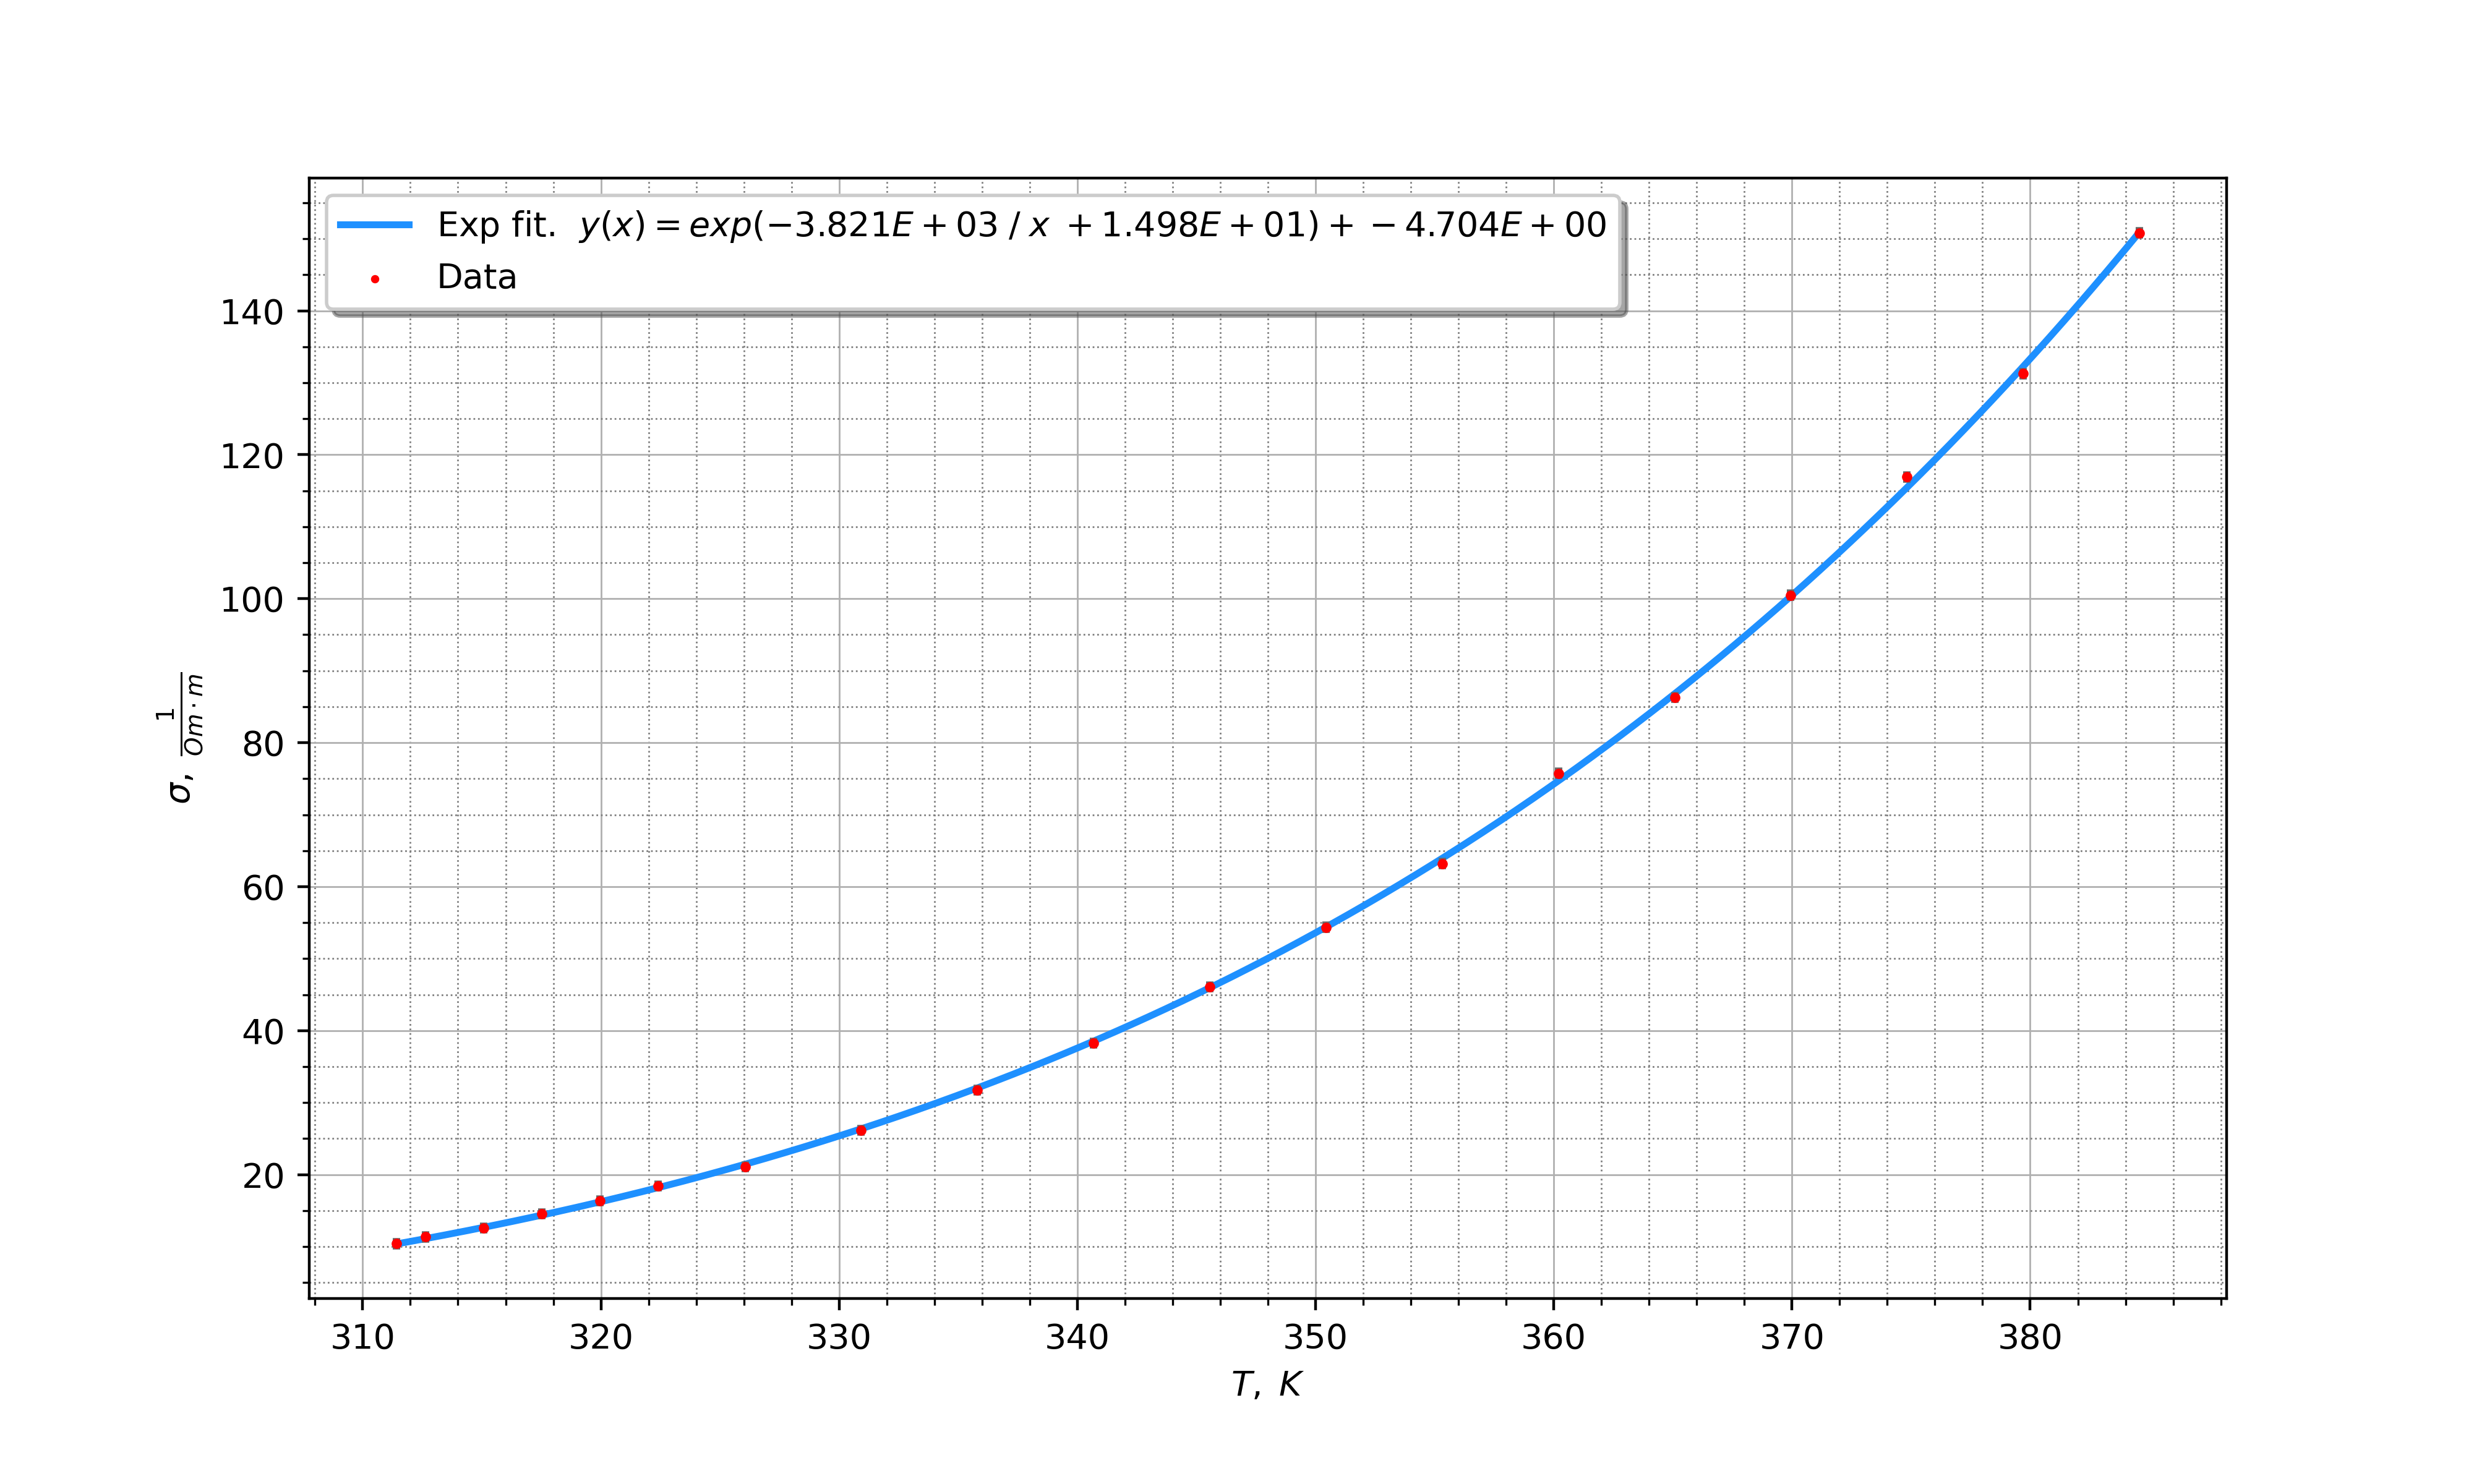
\includegraphics[scale = 0.75]{graph3.png}
        \caption{Зависимость $\sigma(T) $ для полупроводника в режиме постоянного тока}
        \label{gr3}
    \end{center}
\end{figure}

\begin{figure}[h]
    \begin{center}
        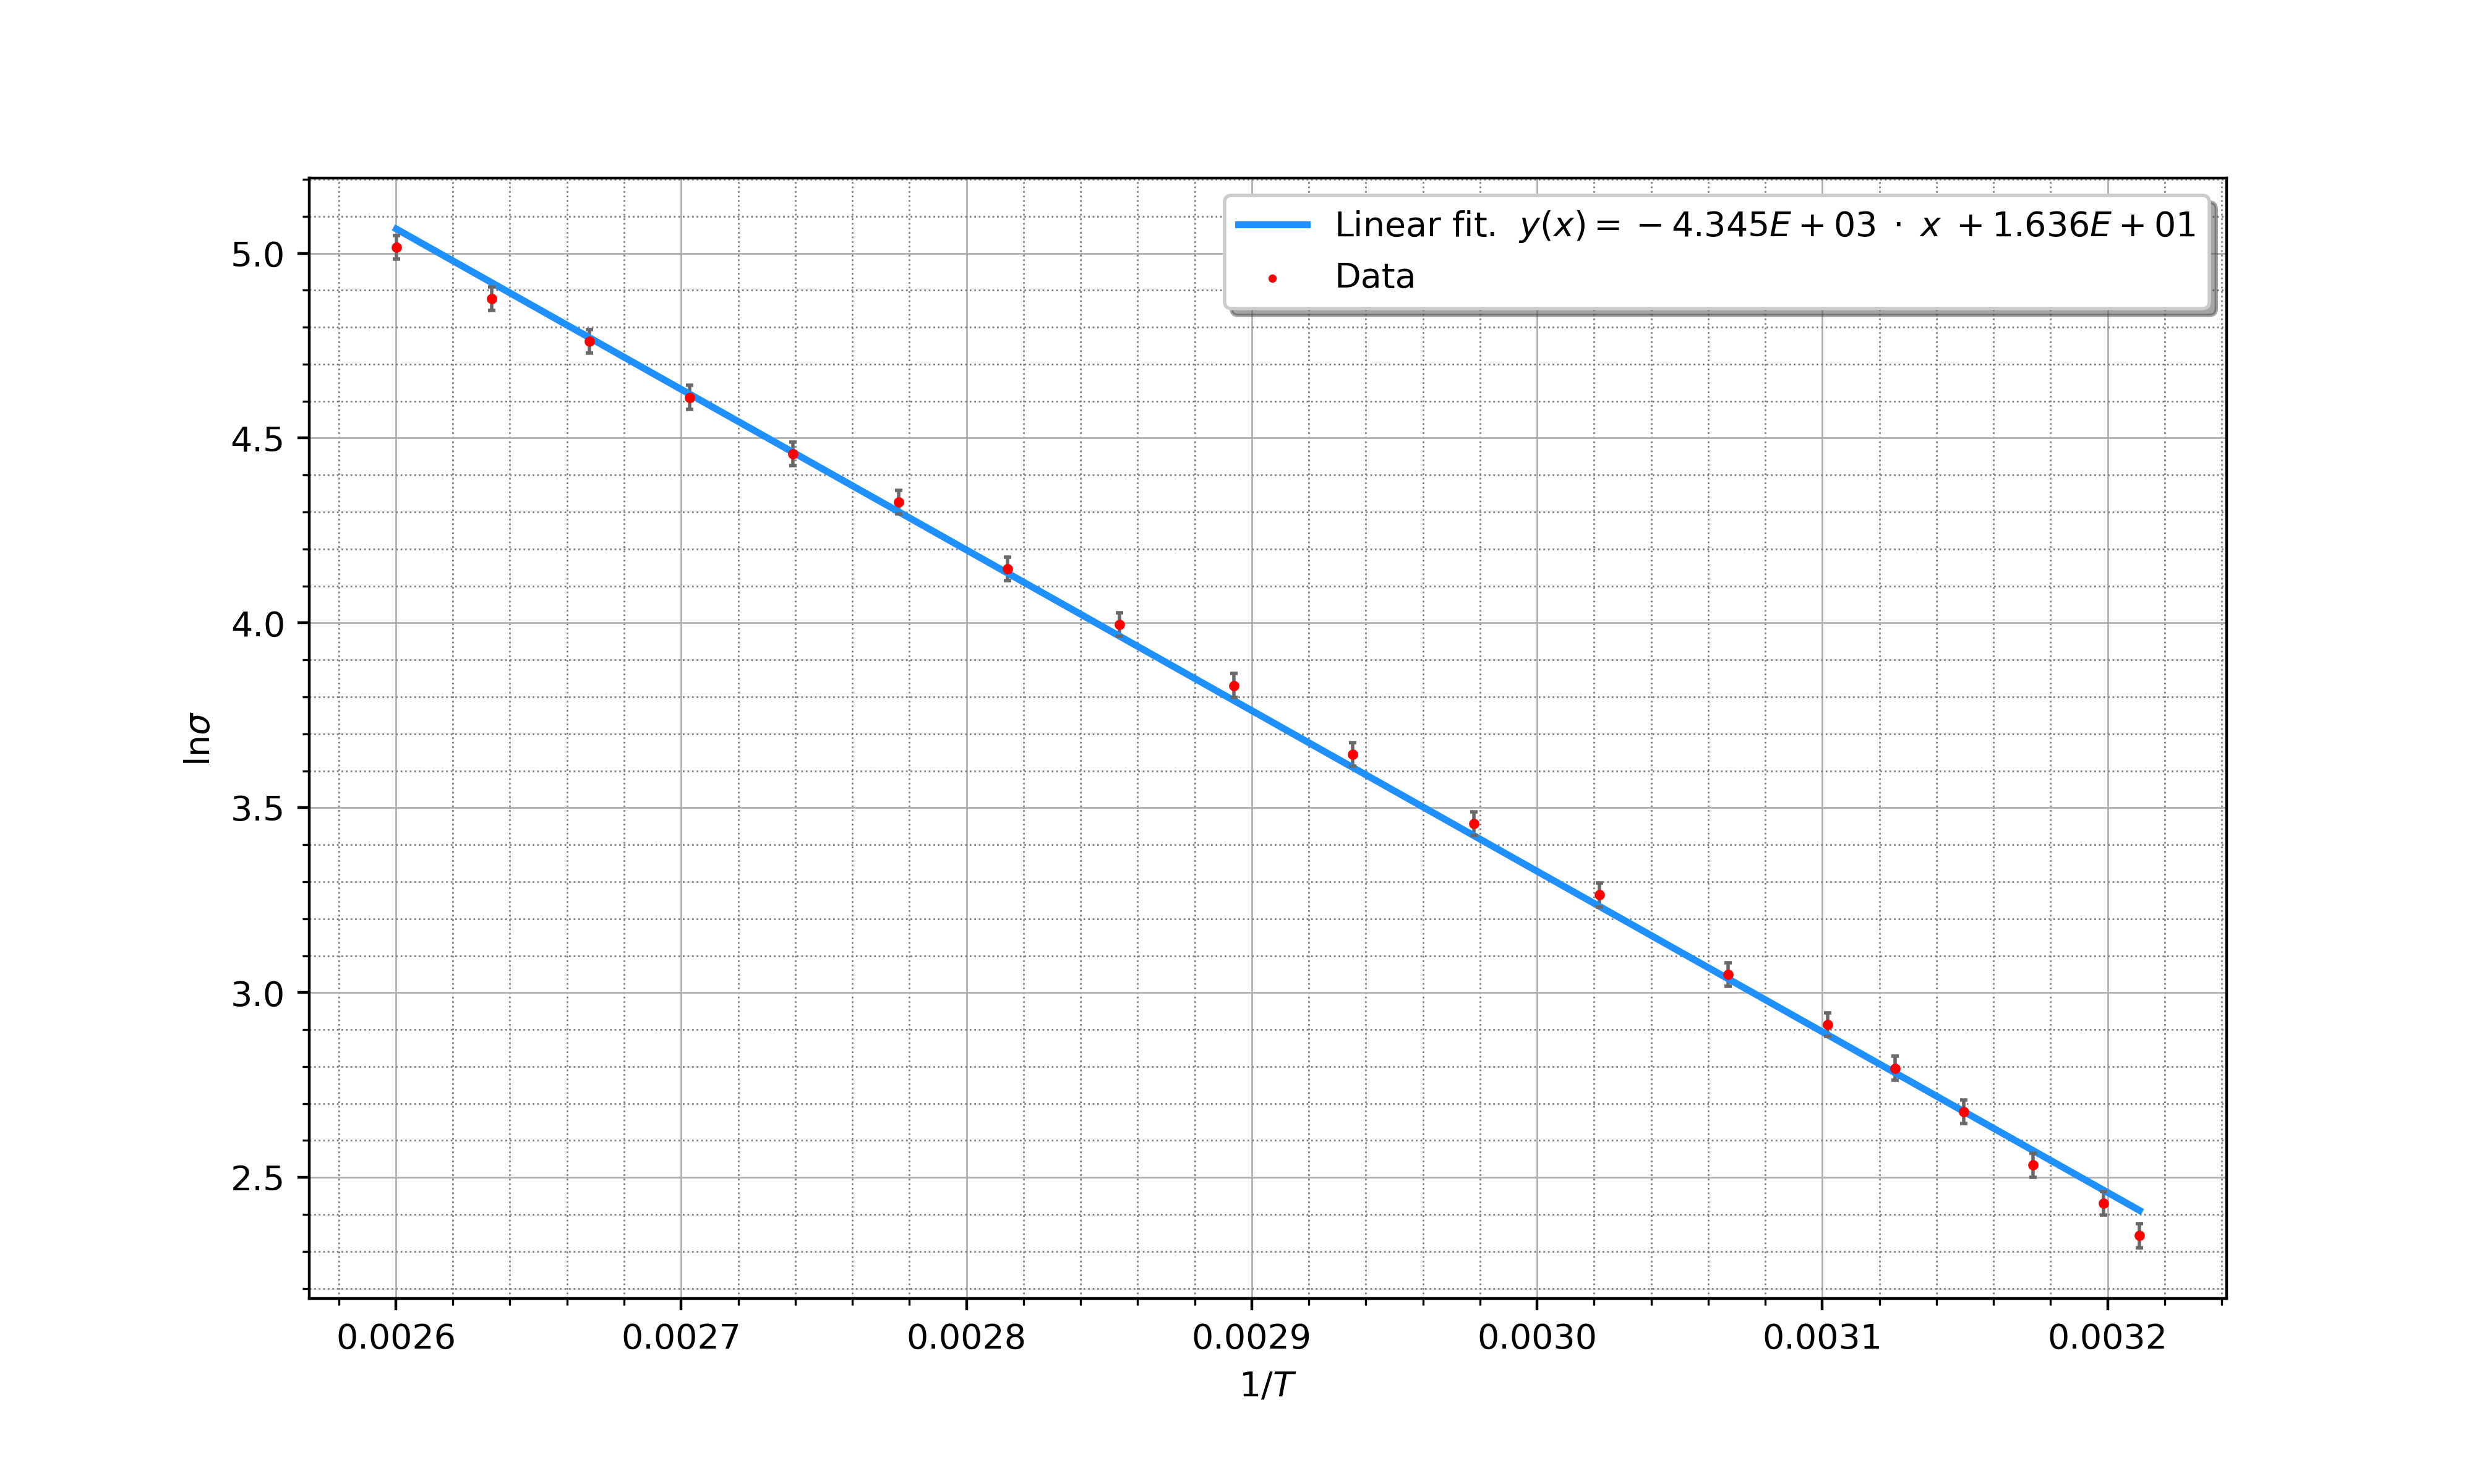
\includegraphics[scale = 0.75]{graph4.png}
        \caption{Зависимость $\ln{\sigma} (1/T)$ для полупроводника в режиме постоянного тока}
        \label{gr4}
    \end{center}
\end{figure}



\begin{figure}[h]
    \begin{center}
        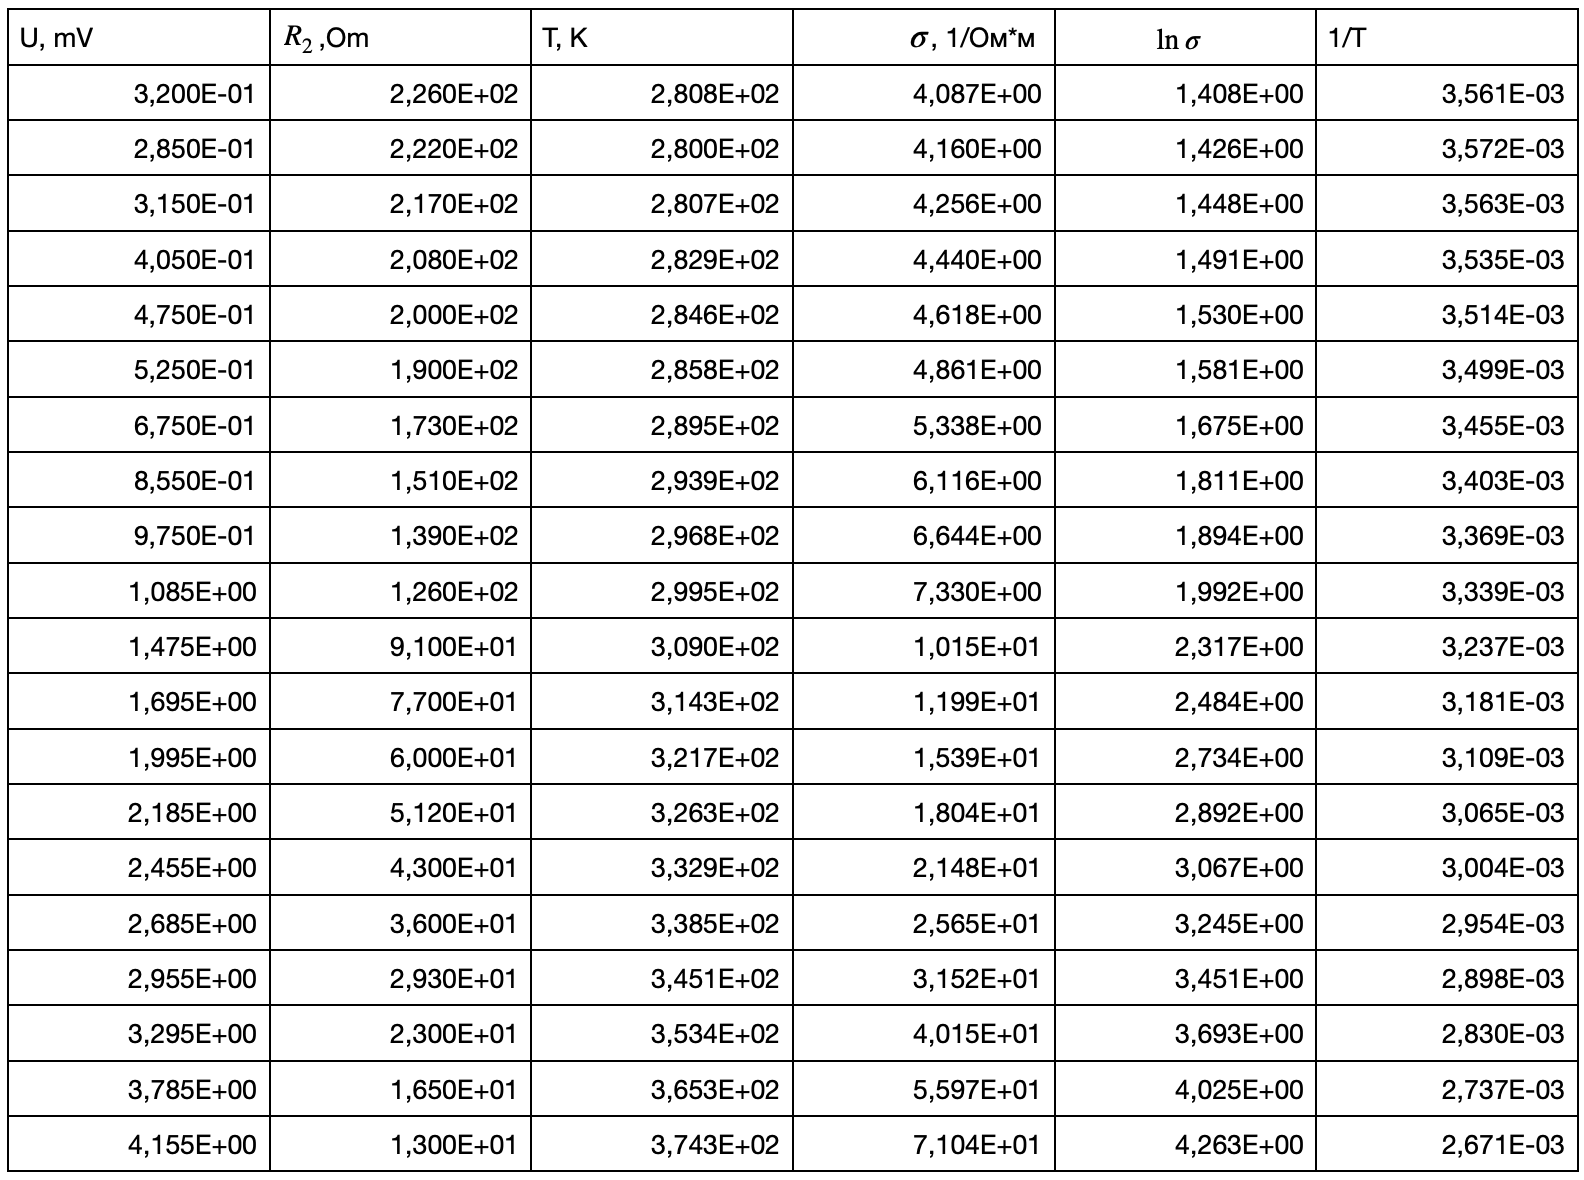
\includegraphics[scale = 0.5]{data.png}
        \caption{Данные исследования в режиме переменного тока}
        \label{data}
    \end{center}
\end{figure}

\begin{figure}[h]
    \begin{center}
        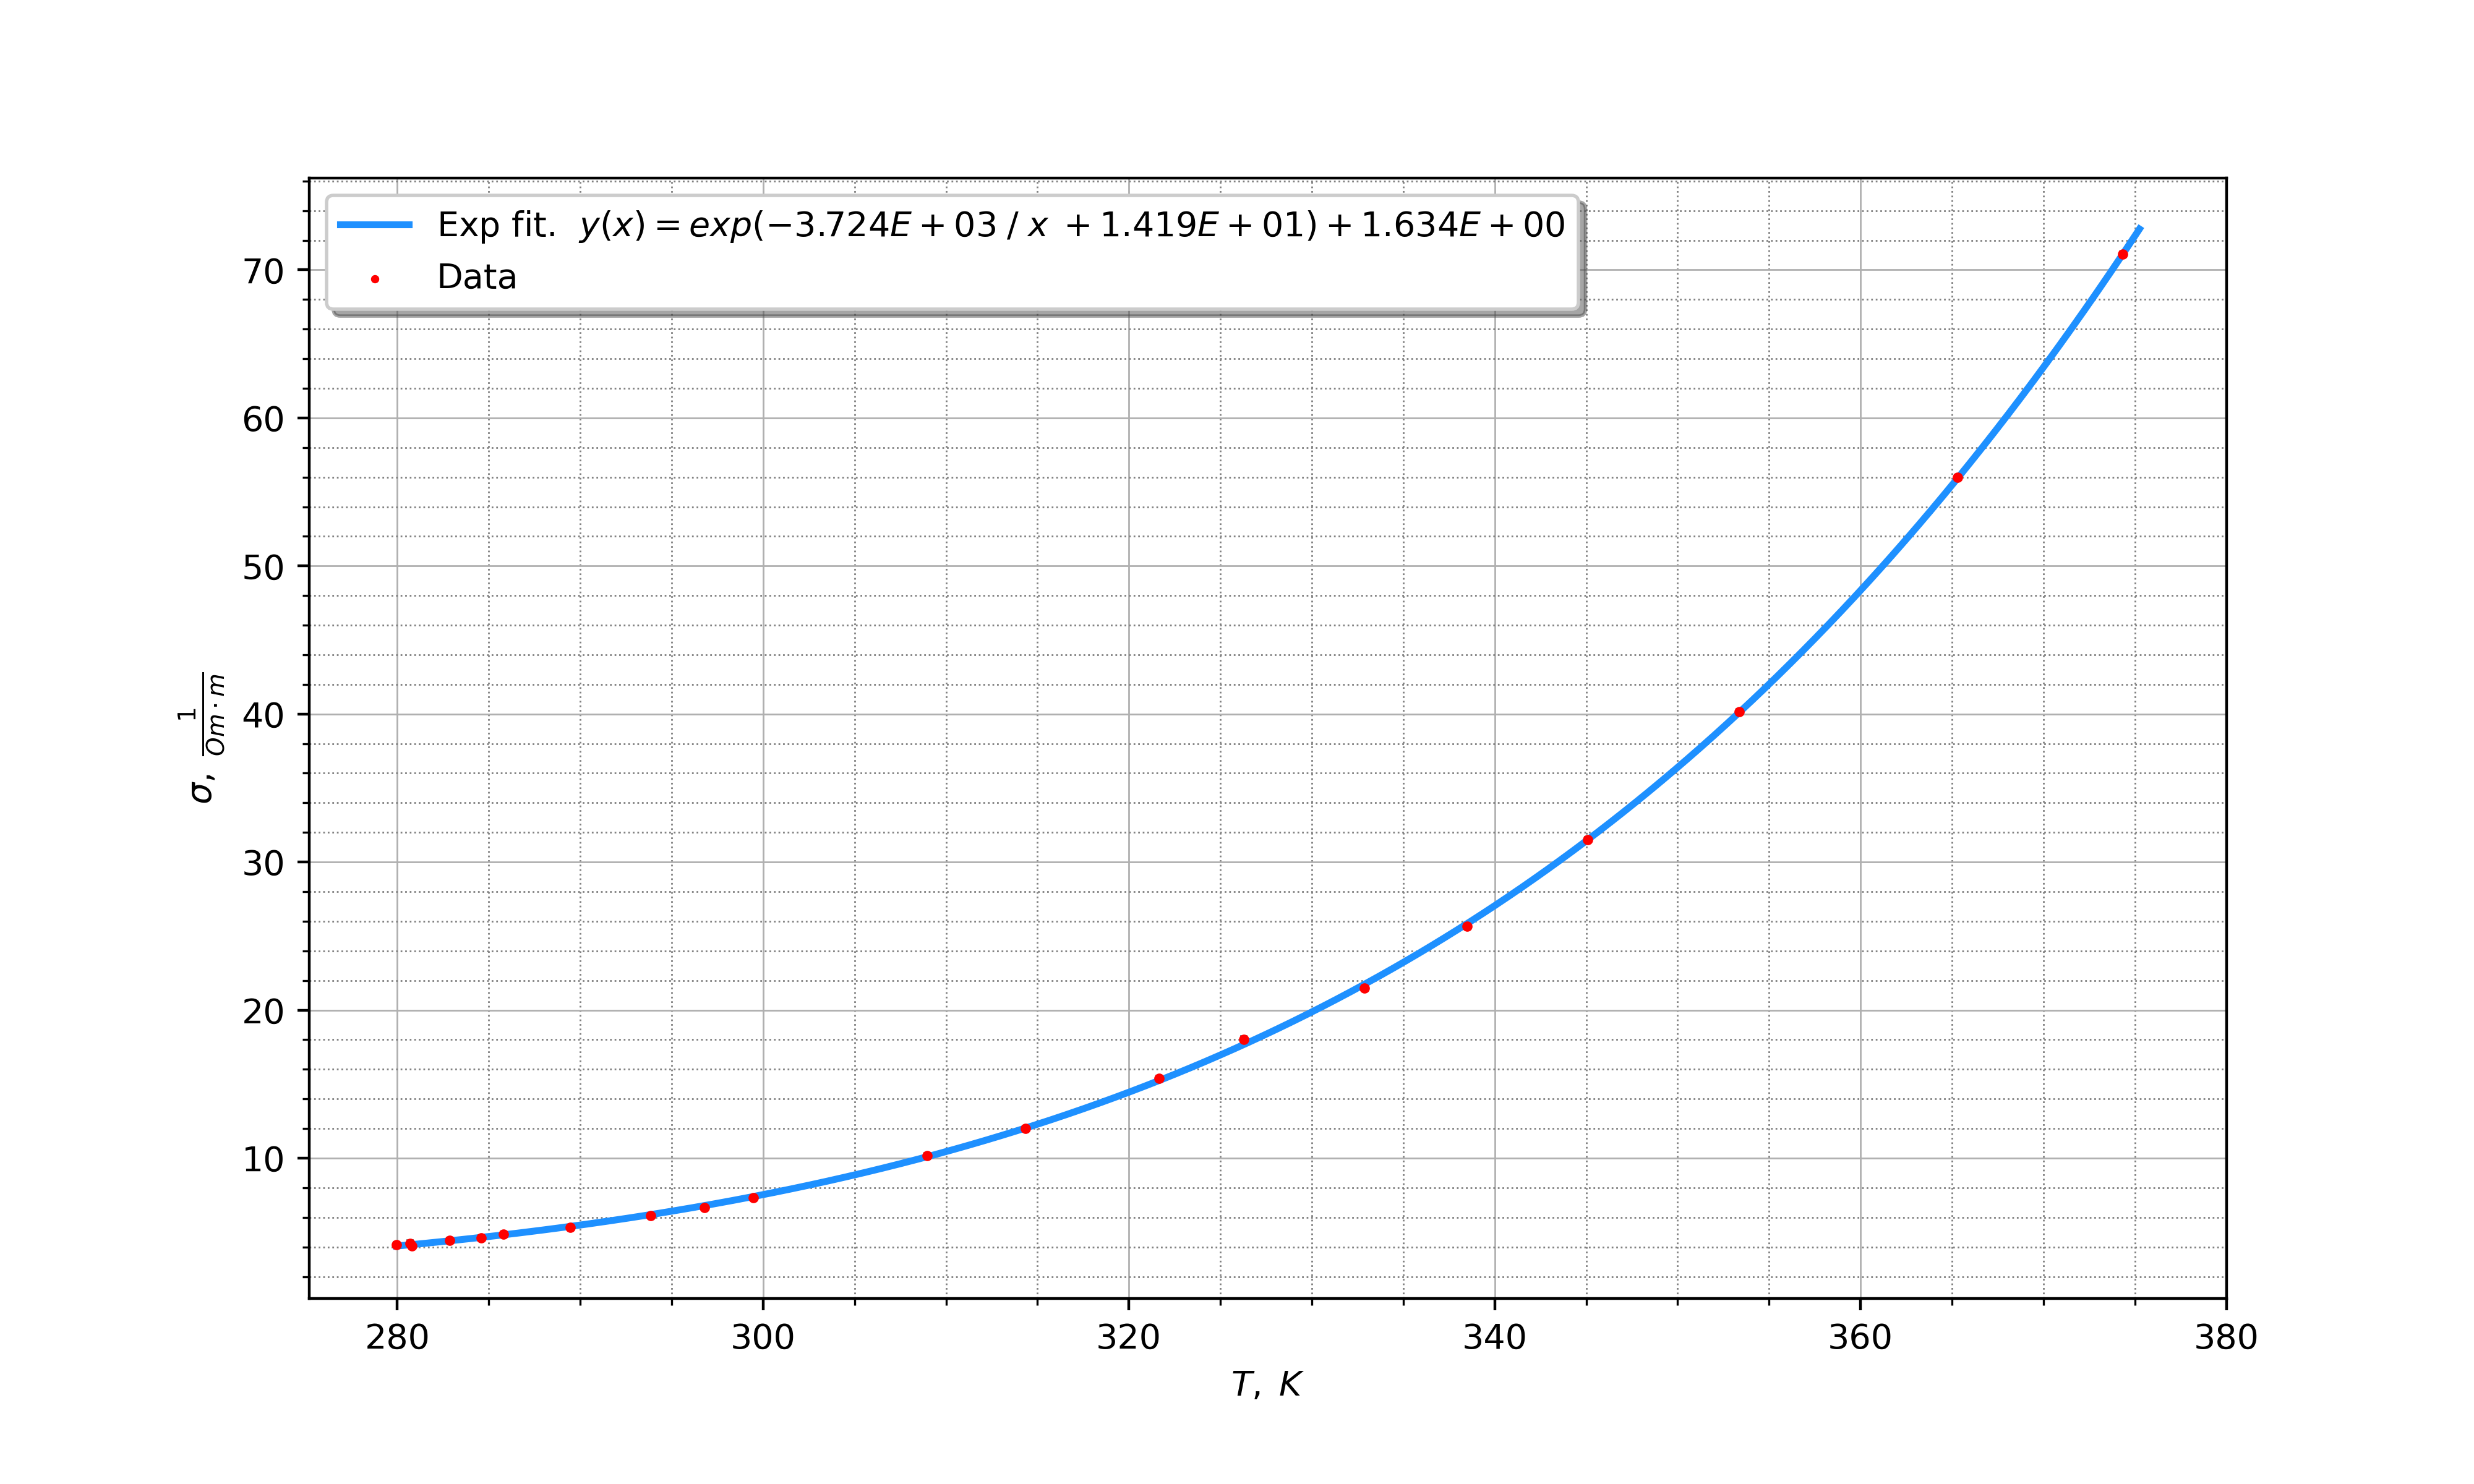
\includegraphics[scale = 0.75]{graph2.png}
        \caption{Зависимость $\sigma(T)$ для полупроводника в режиме переменнрого тока}
        \label{gr2}
    \end{center}
\end{figure}

\begin{figure}[h]
    \begin{center}
        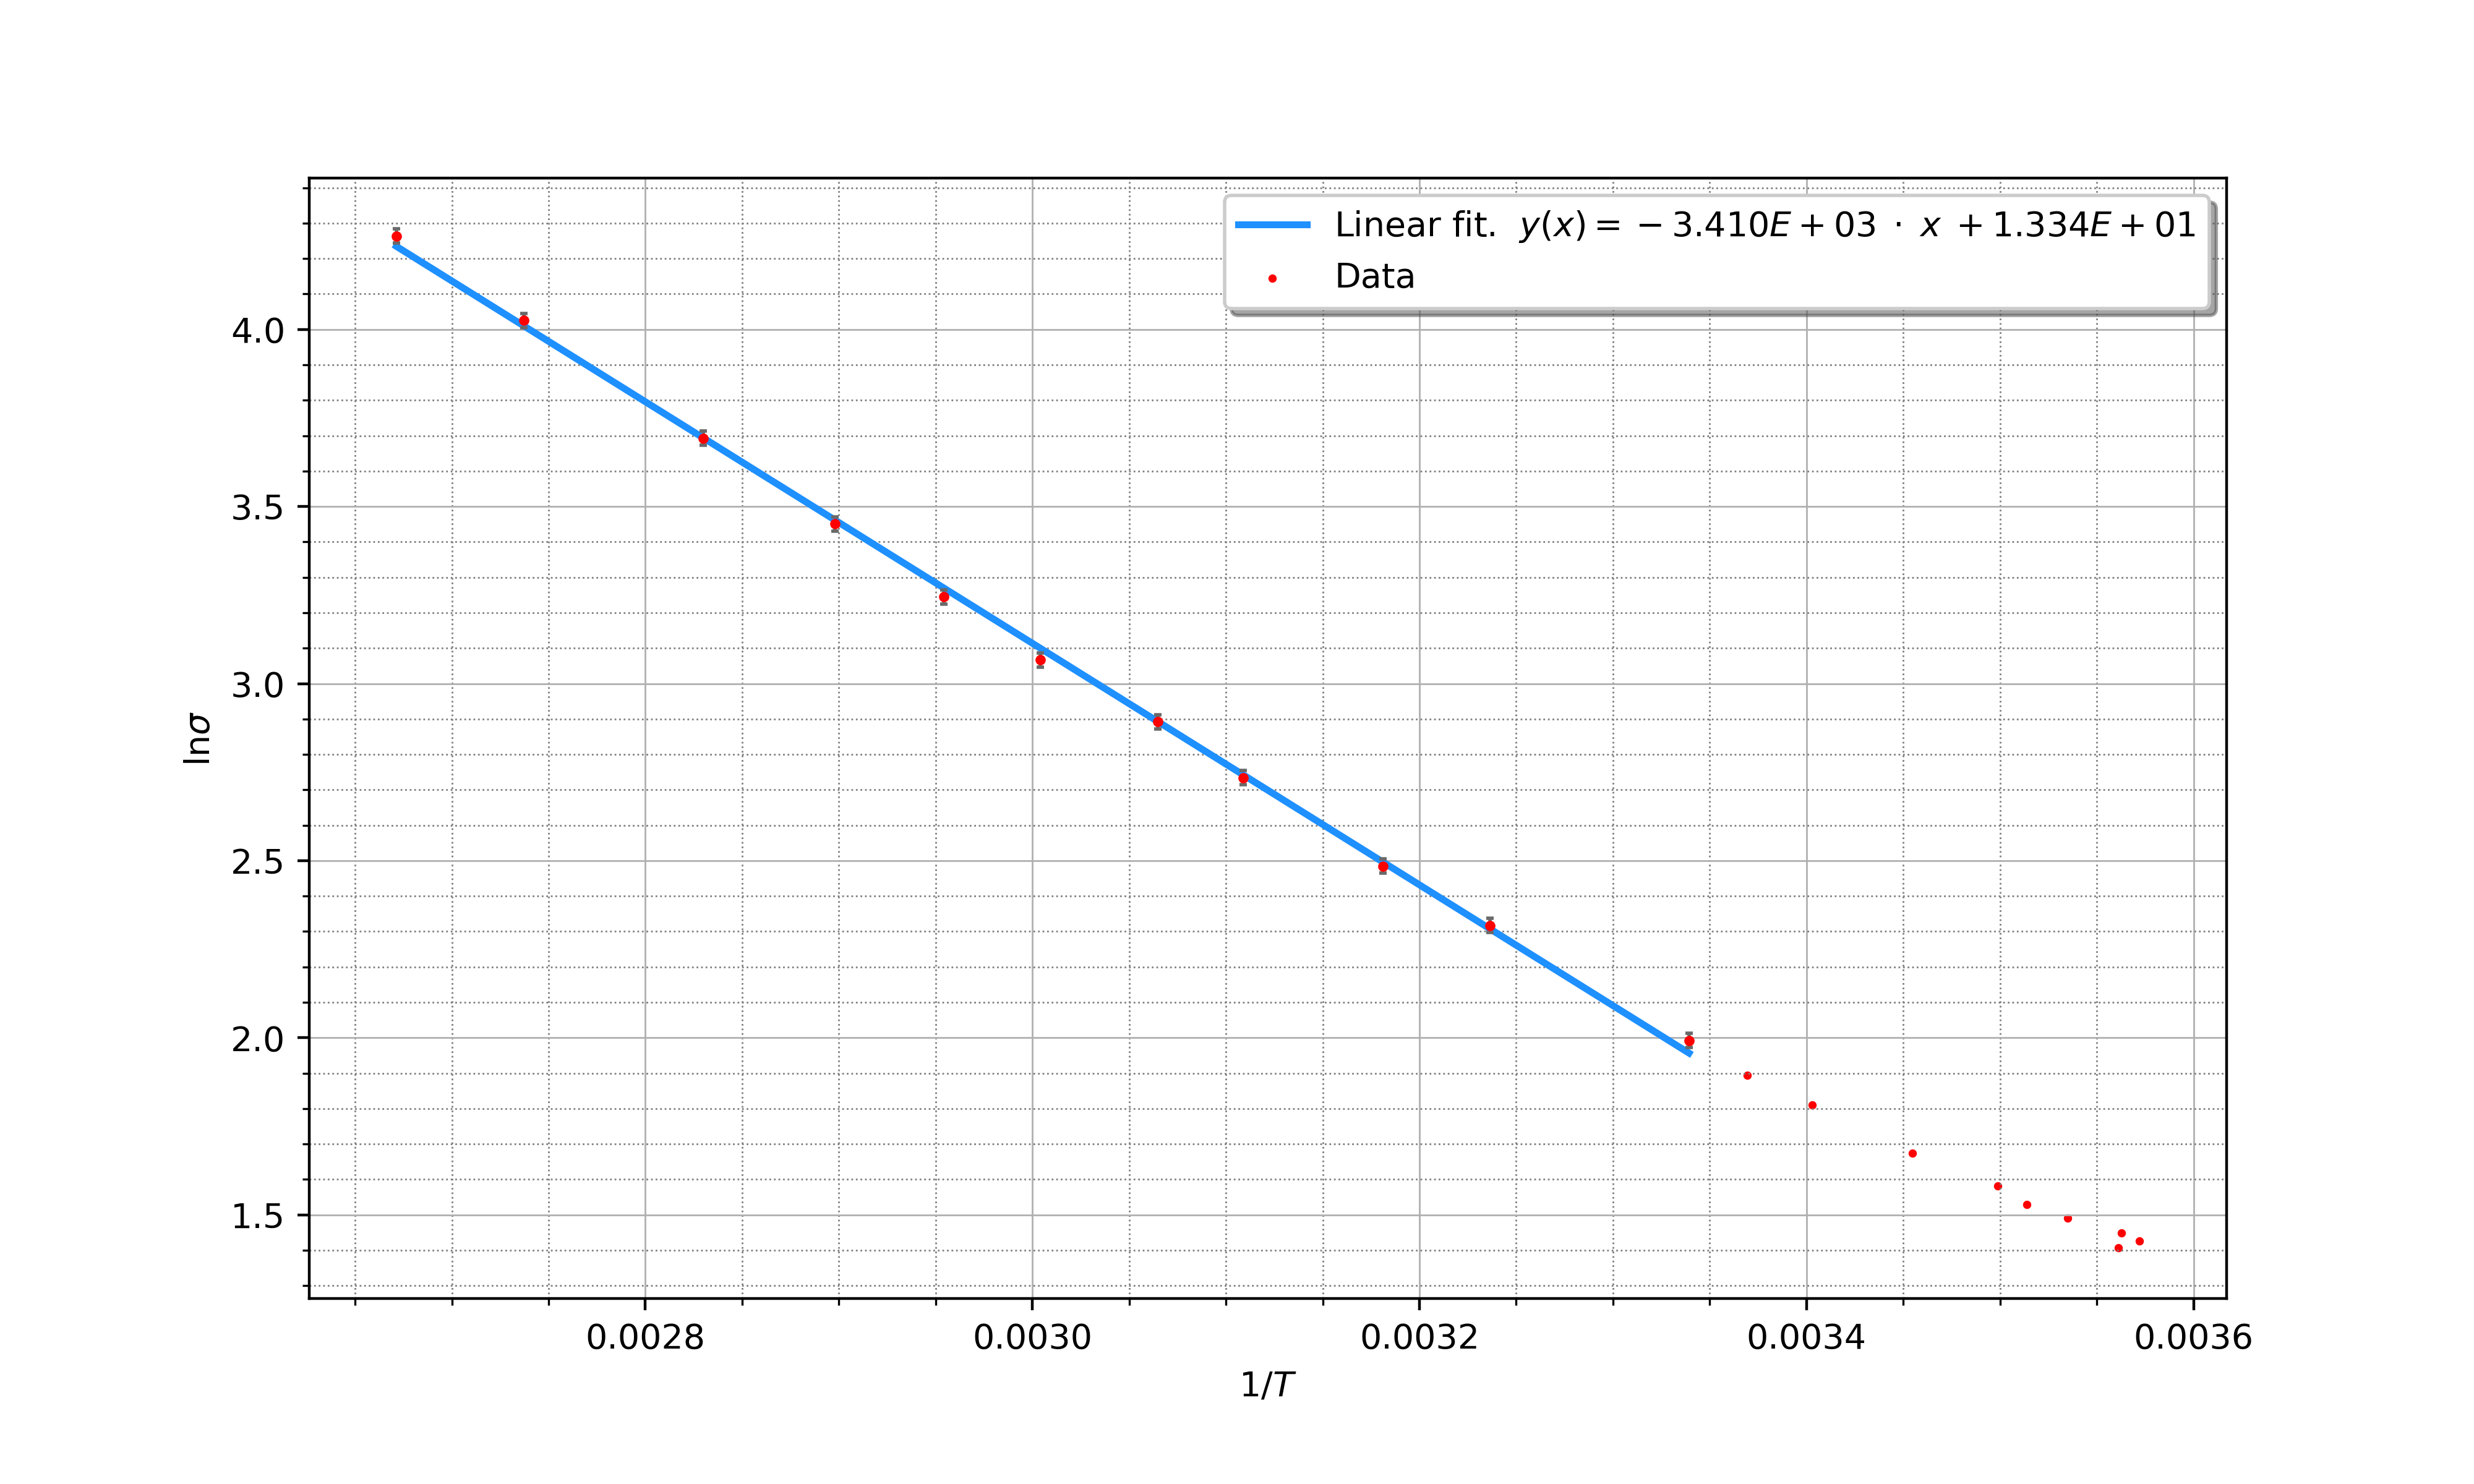
\includegraphics[scale = 0.75]{graph1.png}
        \caption{Зависимость $\ln{\sigma} (1/T)$ полупроводника в режиме переменного тока}
        \label{gr1}
    \end{center}
\end{figure}



\end{document}